\documentclass[a4paper]{article}

%% Language and font encodings
\usepackage[english]{babel}
\usepackage[utf8x]{inputenc}
\usepackage[T1]{fontenc}

%% Sets page size and margins
\usepackage[a4paper,top=3cm,bottom=2cm,left=3cm,right=3cm,marginparwidth=1.75cm]{geometry}

%% Useful packages
\usepackage{amsmath}
\usepackage{graphicx}
\usepackage[colorinlistoftodos]{todonotes}
\usepackage[colorlinks=true, allcolors=blue]{hyperref}
\usepackage{setspace}

% Setup %
%%%%%%%%%%%%%%%%%%%%%%%%%%%%%%%%%%%%%%%%
%%%%%%%%%%%%%%%%%%%%%%%%%%%%%%%%%%%%%%%%
% Cover Page %

\title{Modeling Social Data - Lecture 11, April 14th}
\author{bk2628}

\begin{document}
\maketitle

\doublespacing


\section{Prediction vs Causation}
\subsection{Prediction}
Making a forecast without changing anything.
For example: seeing your neighbor with an umbrella might predict rain

\subsection{Causation}
Make a change in the current scenario, i.e., the current state of the world and anticipate what will happen.

\subsubsection{Reverse causal inference}
Finding the cause of something that has already happened.
For example: what caused my kid to get sick?
Reverse causal inference is generally quite hard.
\subsubsection{Forward causal inference}
Forward causal inference is more "what happens if we do a certain thing?".

\subsubsection{Example : Hospitalization on health}
What's the effect of going to the hospital today on your health tomorrow?
If we try to estimate the above model based on just observational data we may be missing out an unobserved common cause like the health of the person on the day of the hospital visit.

\subsubsection*{Observational estimates}
Let’s say all sick people in our dataset went to the hospital today, and healthy people stayed home \newline
\textbf {Observed difference in health tomorrow}  = (Sick and went to hospital) – (Healthy and stayed home) \newline
\textbf {Observed difference in health tomorrow} = [(Sick and went to hospital) – (Sick if stayed home)] + [(Sick if stayed home) - (Healthy and stayed home)] \newline
\textbf{Causal effect} = (Sick and went to hospital) – (Sick if stayed home) \newline
\textbf {Selection bias} = (Sick if stayed home) - (Healthy and stayed home) \newline
\textbf {Observed difference in health tomorrow} = Casual effect - Selection bias \newline
There is a selection bias in this example because the people visiting the hospital are not random as today's health of the person affects the decision of visiting the hospital today.

\section{Predictive Systems}
Aim : predict the future activity for a user.

\subsection{Search engine example}
Say you wanted to buy a toy from amazon and so, you search for it on Google. Google would show you an ad for Amazon. \newline
But the search results also have Amazon. This raises the following question: \newline
The counterfactual question is "would have i still landed on Amazon.com even without the ad?" \newline
Maybe or maybe not.\newline
There can be hidden causes for the observed results, and ignoring such causes can lead to completely different conclusions. \newline
In the above example, people may have anyway used Amazon.com to order the toy even without the ad. But our observations may suggest that the activity was because of the ad.

\subsection{Simpson's Paradox}
Selection bias can be so large that observational and causal estimates give opposite effects. \newline
(example: going to hospitals makes you less healthy) \newline
Other examples : Comparing an old algorithm with a new one. \newline

\begin{tabular}{c c}
Old Algorithm & New Algorithm  \\
5\%(50/1000) & 5.4\%(54/1000) \newline
\end{tabular} \newline \newline
After dividing the group into low and high activity users \newline
Low activity users \newline
\begin{tabular}{c c}
Old Algorithm & New Algorithm  \\
2.5\%(10/400) & 2\%(4/200) \newline
\end{tabular} \newline \newline
High activity users \newline
\begin{tabular}{c c}
Old Algorithm & New Algorithm  \\
6.6\%(40/600) & 6.2\%(50/800)
\end{tabular} \newline \newline
New algorithm has a better success rate overall but when we divide the data, old algorithm seems to have a higher success rate. \newline
Conclusion: we can add as many variables as we want to the model and different algorithms would perform different under different variables. \newline \newline
\textbf{Going back to the hospital example:} \newline
How can we check if going to the hospital makes you less healthy? \newline
One way is to "clone" the world which means just change the one thing that we want to measure while keeping everything else the same. \newline
Guy goes to the hospital Vs Guy doesn't go to the hospital everything else remains the same. \newline
This works well in theory but how do we actually clone the world? \newline
Take the data set(sick or healthy) and use a coin flip to decide who goes into which version of the world.
Since the decision is based on a coin flip, the expected result would be to get similar samples in both the worlds.\newline
\textbf{Basic identity of causal inference:} \newline
\textbf{observed difference} = causal effect - selection bias \newline
Selection bias is zero since there in no difference, on average, between the two worlds.\newline
\textbf{observed difference} = causal effect

\begin{figure}
	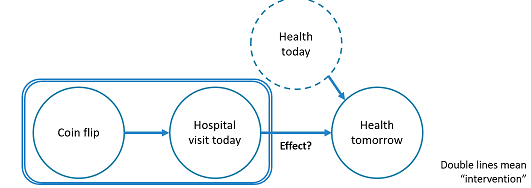
\includegraphics[width = \columnwidth]{image/MSD}
\end{figure}

Random sampling makes sure that health today has no effect on the health tomorrow.
The only thing we are checking is "does going to the hospital today affects you health tomorrow?".

\subsubsection{Experiments : Caveats/Limitations}
\begin{itemize}
\item Randomizations is not always feasible or ethical.
\item Experiments cost a lot of money and time.
\item Anyone can flip a coin, but convincing parallel worlds are hard to simulate.
\item It's inevitable that some people would deviate from their random assignments.
\end{itemize}

\subsubsection{Experiment : Experimental drug trial}
Two goals for this experiment:\newline
\textbf{1) Internal Validity:}
Could anything other than the treatment have produced results?\newline
One cause could be that doctors gave the medicine to some special patients, thus breaking the randomization. \newline
\textbf{2) External Validity:}
Do the results of the experiment hold in a setting that we care about? \newline
Would the medicine be as successful in the real world as it was in the clinical trial? \newline
One example is birth control pills which may not be as effective in the real world as they are during the test on account of people forgetting to take them on same days.

\section{How we conduct behavioral experiments?}
\subsection{Lab Experiment}
\subsubsection{Better internal validity}
\begin{itemize}
\item Greatest procedural control: we can define the setting the experiment takes place.
\item Can carefully curate situations
\end{itemize}

\subsubsection{Less external validity}
\begin{itemize}
\item Artificial context, simple tasks : \newline
The user may have behaved differently in a "natural" environment.
\item Demand effects 
\item Homogeneous (WEIRD) subject pool \newline
WEIRD stands for Western, educated, and from industrialized, rich, and democratic.
\item Time/scale limitations
\end{itemize}

\subsection{Field Experiment}
\subsubsection{Better generalization}
\begin{itemize}
\item Experiment findings apply to at least one real world setting
\end{itemize}

\subsubsection{But:}
\begin{itemize}
\item Less Control, more potential confounds
\item Demand of experiment conflicts with goals of real organizations
\item More effort to conduct and manage
\item More room for error
\end{itemize}

\section{Examples of Causal Inference}
\subsection{Natural Experiments:}
Sometimes nature runs experiment for us, e.g.:

\subsubsection{As-if random:} People are randomly exposed to water sources (Snow, 1854)
\subsubsection{Instrumental variables:} An instrument independently shifts the distribution of a treatment.
Example: A lottery influences military service (Angrist, 1990)

What can we try to infer?
1) Effect of lottery in making people join the military.
2) What would be somebody's future earnings if your name was called in the lottery?

\subsubsection*{Natural experiments: Caveats}
\begin{itemize}
\item Good natural experiments are hard to find.
\item They may have many (untested) assumptions.
\item The treated population may not be the one of interest.
\end{itemize}


\end{document}